\documentclass{beamer} %[handout] pour supprimer la barre de navigation mais \pause ne fonctionne pas dans ce mode
\usepackage[frenchb]{babel}
\usepackage[T1]{fontenc}
\usepackage[utf8]{inputenc}


\usetheme{Warsaw}

\title[Détection-suivi de véhicule]{Détection et suivi de véhicule par caméra embarquée}
\author{Brehmer Alexandre \and Cluizel Christophe}
\institute{INSA Rouen}
\date{\today}

%ajoute la numérotation des pages et nombre pages total
\addtobeamertemplate{footline}{\hfill\insertframenumber/\inserttotalframenumber\hspace{2em}\null}

%indiquer le chemin du dossier des images
\graphicspath{{}{image/}}

\usepackage{array}
\usepackage{url}
\usepackage{hyperref}


\begin{document}
  \begin{frame}[plain]
  \titlepage
  \end{frame}

  \AtBeginSection[]
  {
    \begin{frame}
    \frametitle{Sommaire}
    \tableofcontents[currentsection, hideothersubsections]

    \end{frame}
  }

  \section{Introduction}
\begin{frame}
    \frametitle{Introduction}

    \begin{center}
        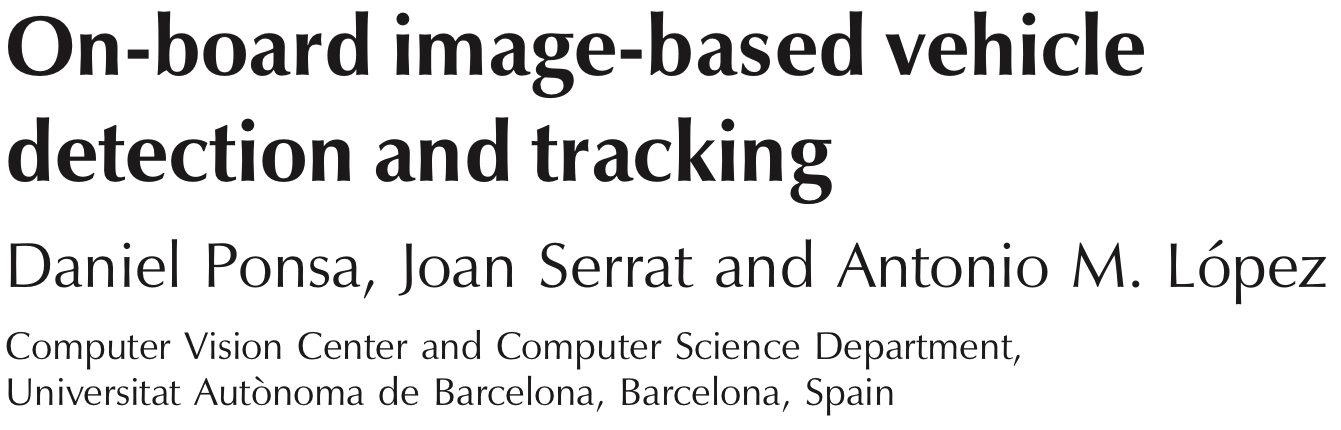
\includegraphics[width=8cm]{titre.png} \\
        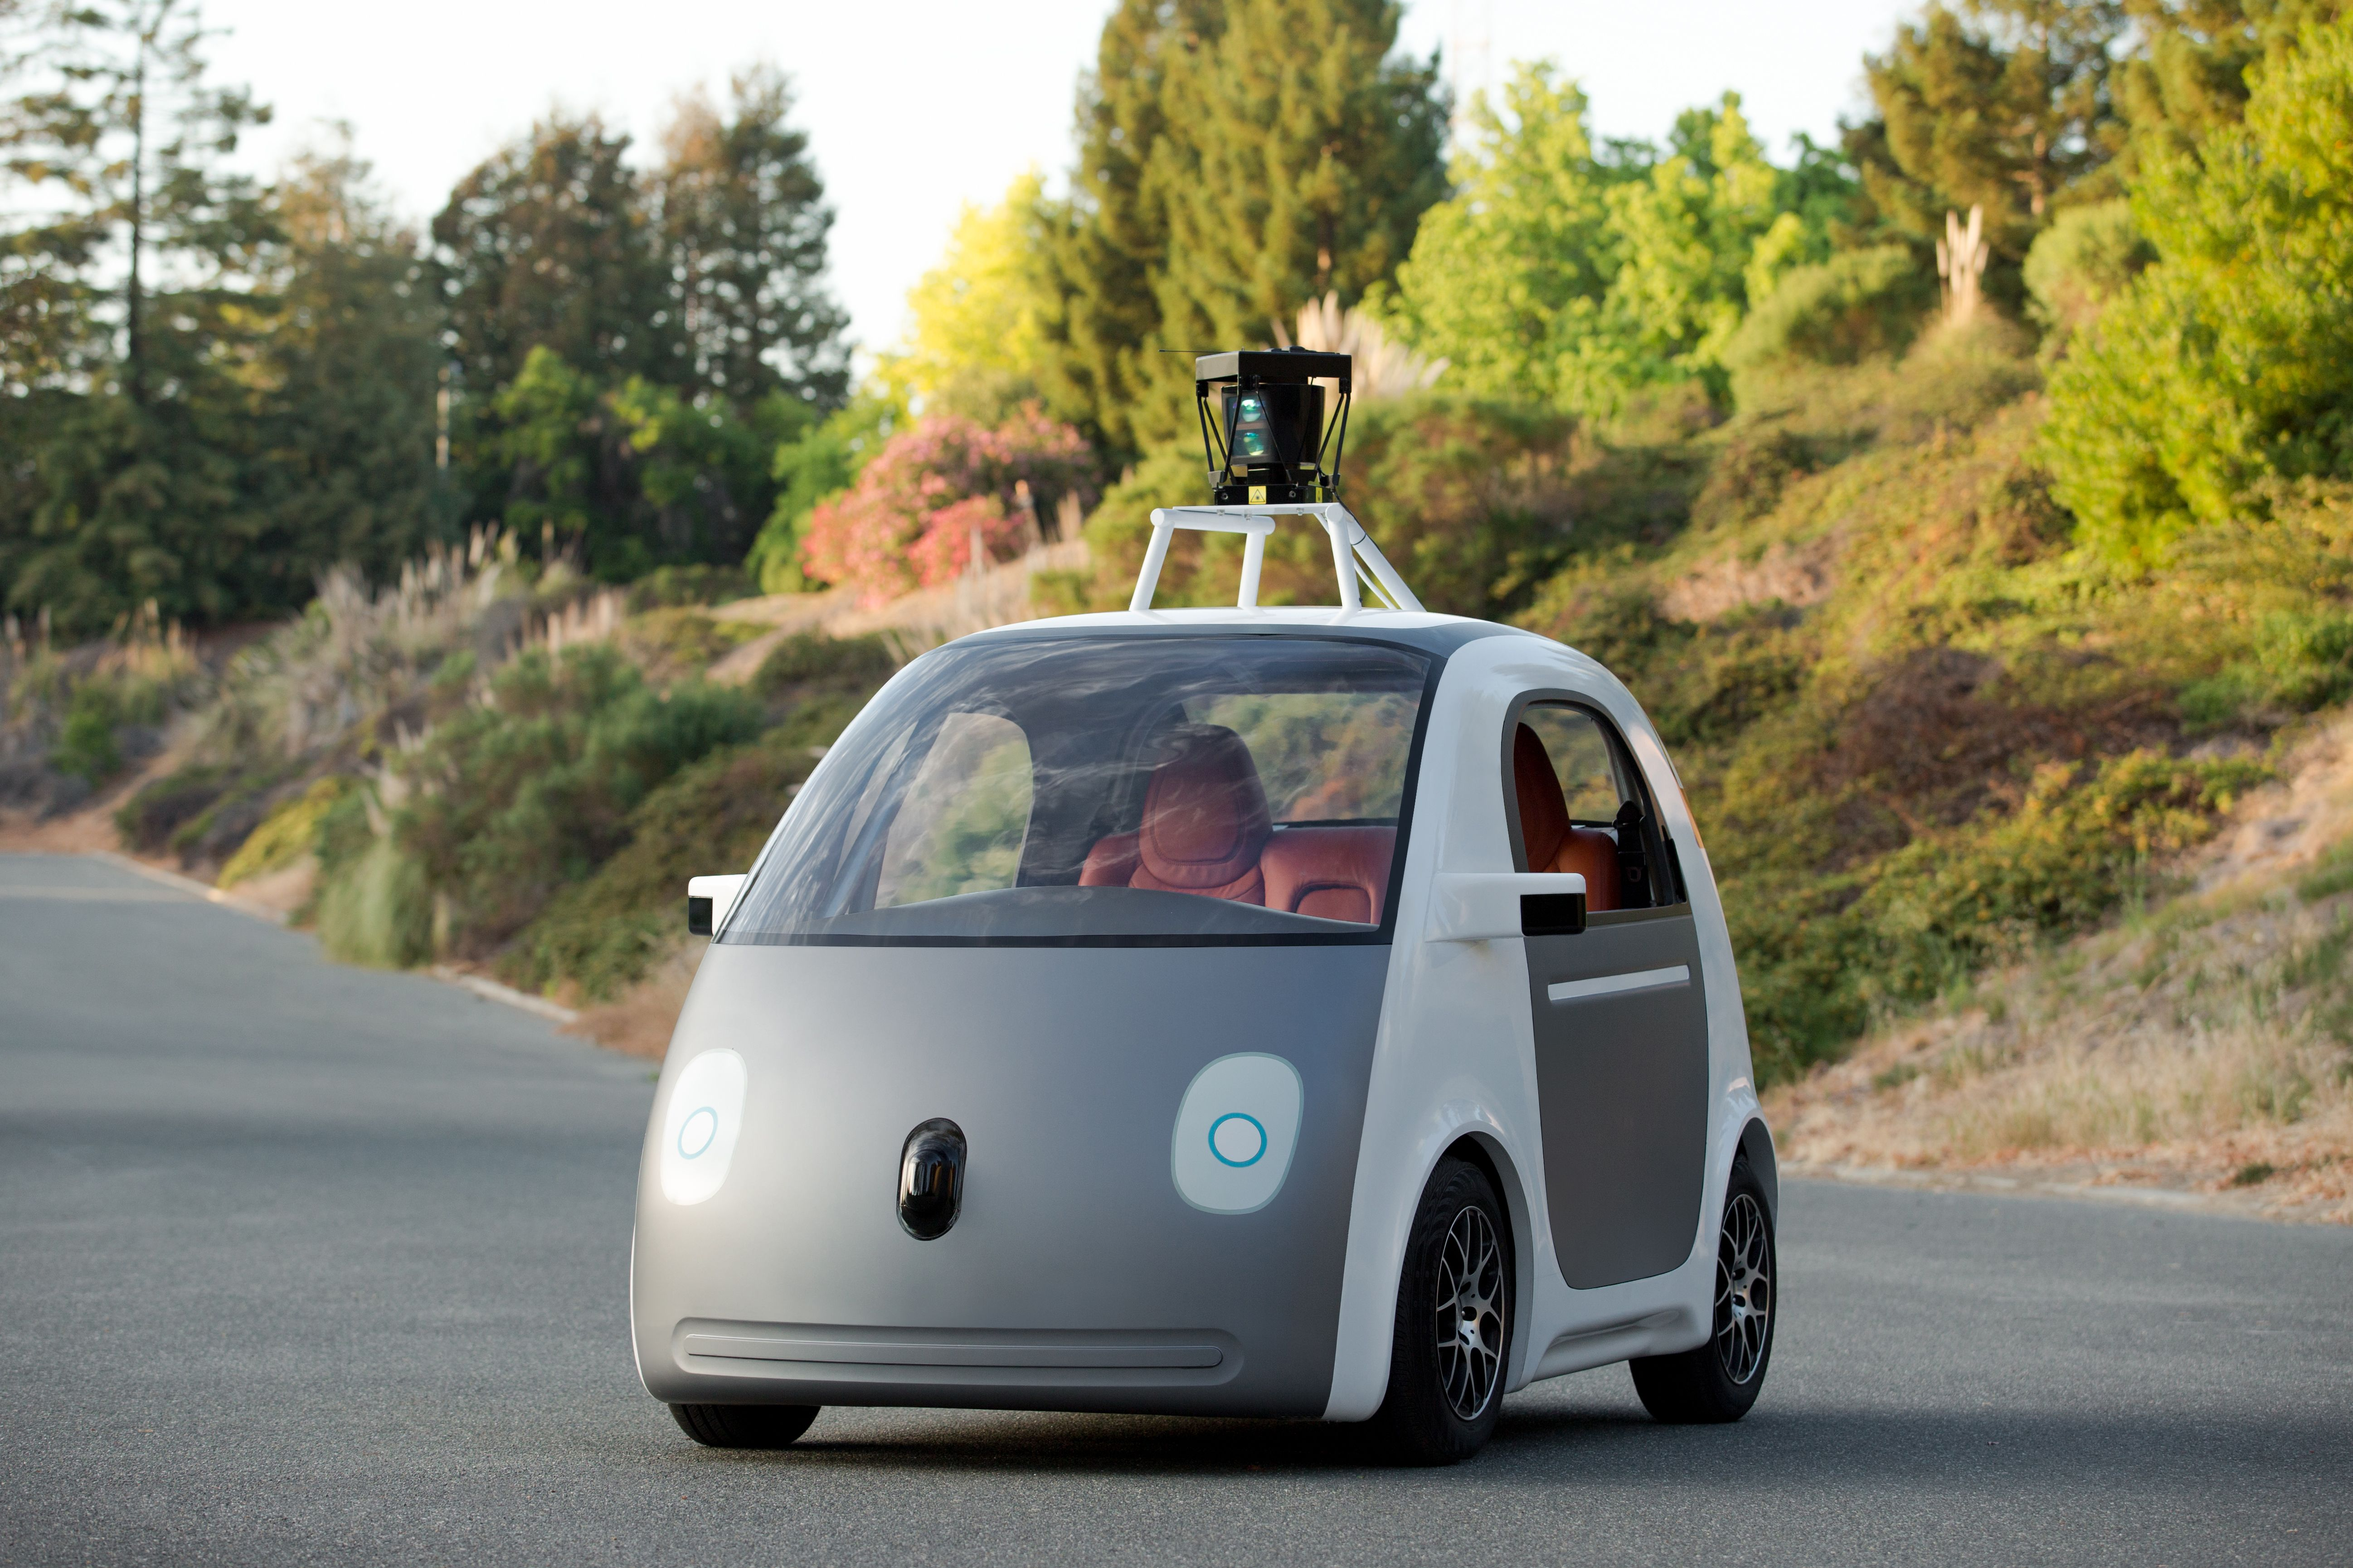
\includegraphics[width=5cm]{google_car.jpg}
    \end{center}
\end{frame}

  \section{Objectifs de l'article}
\begin{frame}
\frametitle{Objectifs de l'article}
Présentation des systèmes :
\begin{itemize}
\item de détection de la route.
\item de reconnaissance de véhicule.
\item d'estimation des positions des véhicules.
\end{itemize}
\end{frame}

  \section{État de l'art}

% slide detection de vehicule
\subsection{Détection du véhicule}
\begin{frame}
\frametitle{État de l'art}

Détection du véhicule. Méthode ``naïve'':
\begin{itemize}
    \item recherche de caractéristiques bas-niveau (ombres, arêtes, symétries…)
    \item peu fiable avec beaucoup de faux-positifs et sensible aux variations lumineuses
    \item rapide et utilisée pour présélectionner des zones de recherche
\end{itemize}
\end{frame}

\begin{frame}
\frametitle{État de l'art}

Détection du véhicule. Méthode ``lourde'':
\begin{itemize}
    \item machine learning (SVM et NN) sur l'ensemble de l'image avec des descripteurs (orientation des arêtes, textures…)
    \item lourd en calculs
    \item utilisée après une présélection de zones
\end{itemize}
\end{frame}

% slide detection de marquage au sol
\subsection{Détection du marquage au sol}
\begin{frame}
\frametitle{État de l'art}

Détection de marquage au sol:
\begin{itemize}
    \item technique la plus étudiée car indispensable au guidage latéral
    \item nombreux problèmes de détection (ombres, variations de contraste, marquage effacé, obstruction par véhicule…)
    \item détection de zones où des lignes peuvent être présentes (détection de Canny)
    \item application d'un modèle mathématiques (ligne droite, quadratique…)
    \item tracking pour accélérer le temps de calcul et la continuité
\end{itemize}

\end{frame}

% slide combinaison des 2 methodes ci-dessus
\subsection{Combinaison des 2 méthodes précédentes}
\begin{frame}
\frametitle{État de l'art}

Combinaison des 2 techniques précédentes:
\begin{itemize}
    \item utiliser les 2 techniques séparément et combiner leurs résultats
    \item utiliser le marquage pour assister le processus de détection de véhicule
    \item utiliser les 2 techniques simultanément pour ``s'auto-optimiser''
\end{itemize}

\end{frame}

  \section{Présentation de la solution de l'article}


%--------- lane-marking  ----------------
\subsection{Détection de la route}
\begin{frame}
\frametitle{Présentation de la solution de l'article}

Détection du tracé de la route
\begin{center}
  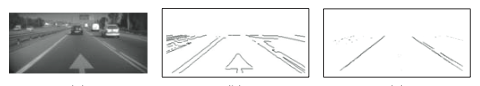
\includegraphics[width=9cm]{image/marquage.png}\\
  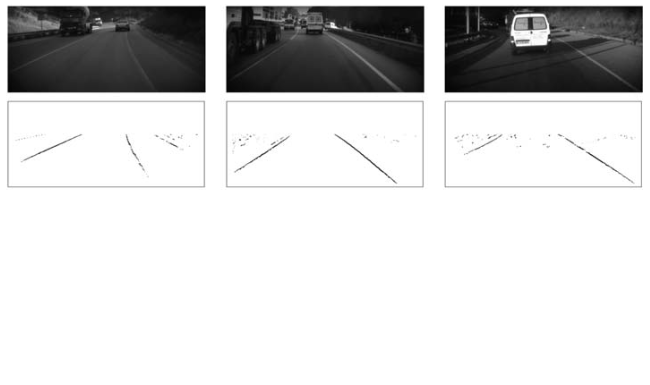
\includegraphics[width=9cm]{image/lignes.png}
\end{center}

\end{frame}

%--------- Reduction du nombre de zones de recherche  ----------------
\subsection{Reconnaissance des véhicules}
\begin{frame}
\frametitle{Présentation de la solution de l'article}

Réduction du nombre de zones de recherche
\begin{center}
  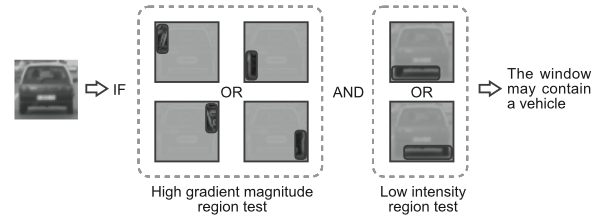
\includegraphics[width=9cm]{image/fenetreVehicule.png}
\end{center}

\end{frame}

%--------- Processus de détection  ----------------
\subsection{Reconnaissance des véhicules}
\begin{frame}
\frametitle{Présentation de la solution de l'article}

Processus de détection de véhicule
\begin{center}
  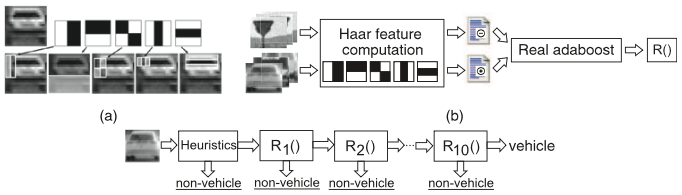
\includegraphics[width=11cm]{image/detectionVehicule.png}
\end{center}

\end{frame}

%--------- Positionnement du vehicule  ----------------
\subsection{Localisation du véhicule}
\begin{frame}
\frametitle{Présentation de la solution de l'article}

Projection d'un plan 2D/3D
\begin{center}
  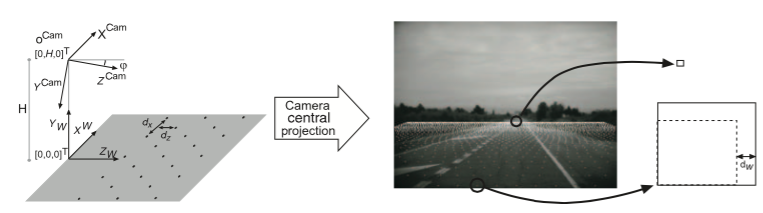
\includegraphics[width=11cm]{image/position.png}
\end{center}

\end{frame}
  \section{Présentation des résultats}
\begin{frame}
\frametitle{Présentation des résultats}

\end{frame}

  \section{Conclusion}
\begin{frame}
\frametitle{Conclusion}

\end{frame}


\end{document}
